\documentclass{article}
\usepackage[utf8]{inputenc}

\title{Recurrent Neural Networks}
\author{Justin Zhang }
\date{February 2018}

\usepackage{natbib}
\usepackage{graphicx}
\usepackage{epigraph}
\usepackage{float}

\begin{document}

\maketitle

\section{Introduction}
Recurrent Neural Networks (RNNs) are a type of neural network that specializes on sequential data; that is, data that is dependant on prior data. For instance, RNNs are often used for natural language processing, because a given word is more likely to appear depending on the prior words. In this vein, RNNs have been applied to tasks like machine translation, image caption generation, and word prediction. However, RNNs have also seen moderate successes in image generation and audio generation.

\section{Intuition}
    In order to handle sequential data, a recurrent neural network has to be able to input a tensor of variable lengths. To do this, we design a \textit{cell} that can be "unrolled," or looped.
    \begin{figure}[H]
        \centerline{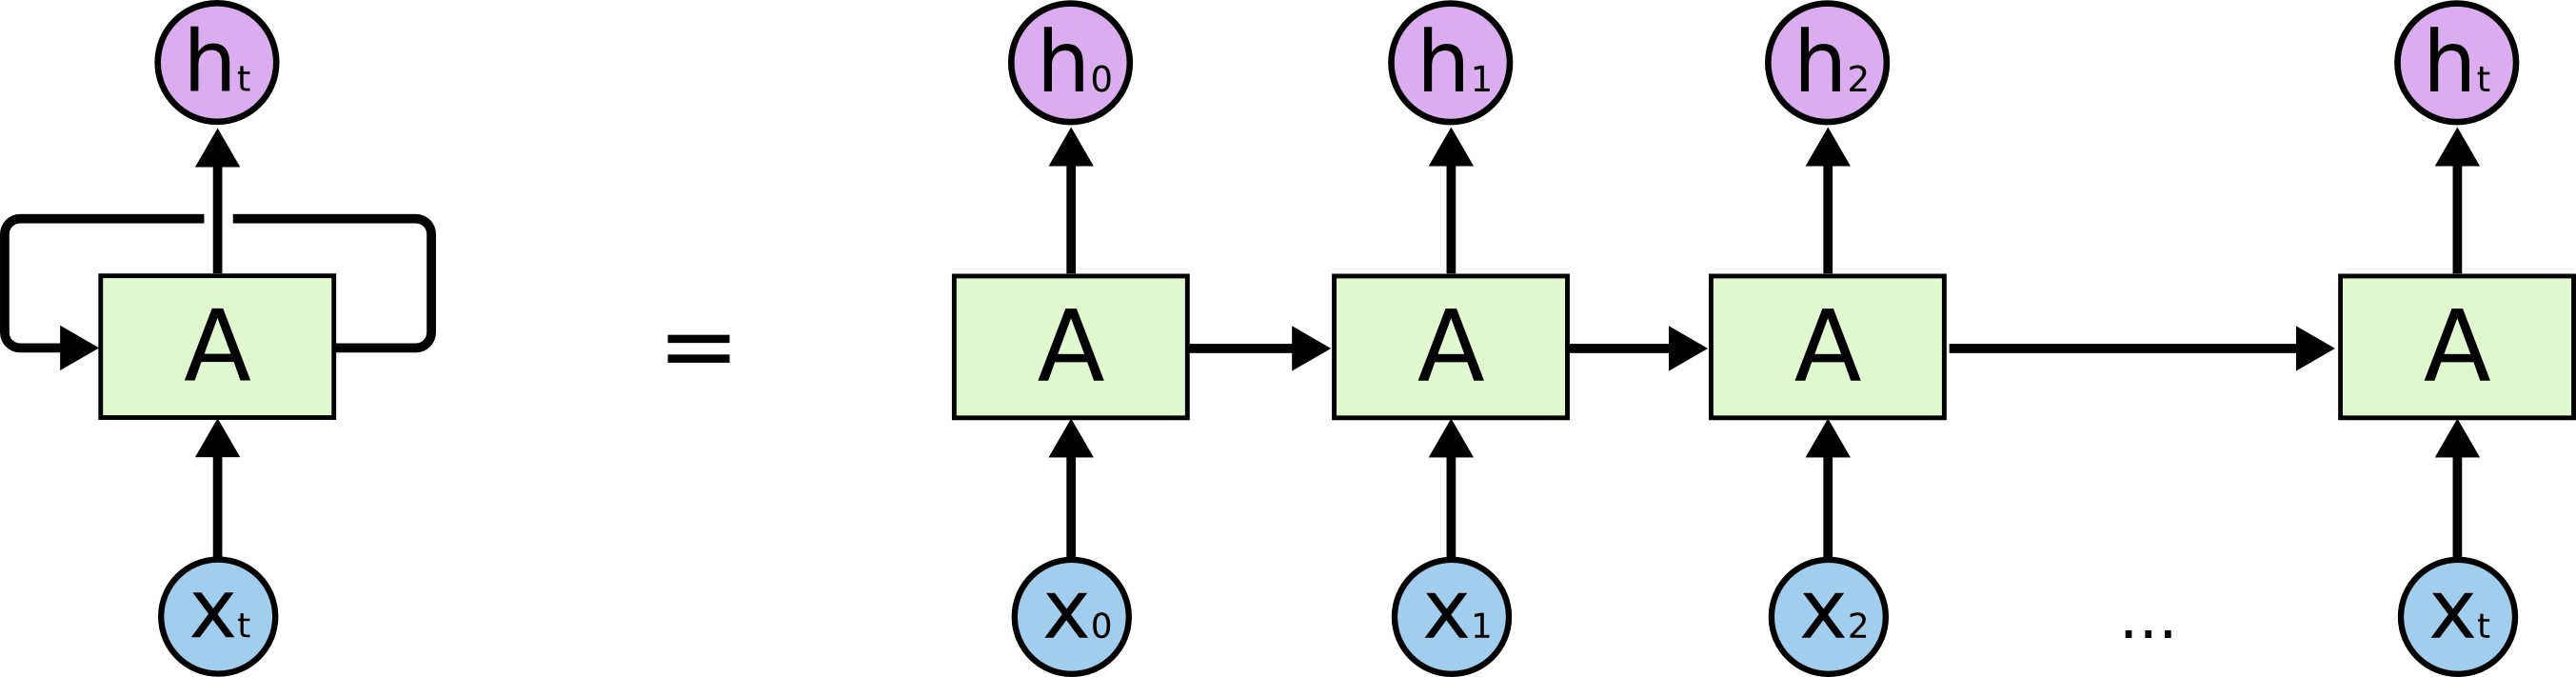
\includegraphics[scale=0.3]{RNN-unrolled.png}}
        \caption{An unrolled RNN.}
        \label{fig:rnn}
    \end{figure}
    This RNN also has to be able to use the previous context as a prior to the next output. This architecture alone works well with the immediate previous context; however, not so much for long-term dependencies.
    
    Let's take a word predictor, for instance. Given part of a sentence, predict the next word. This structure would work quite well for a sentence like "I ate some delicious ice \_\_\_\_"; "ice" provides a significant cue that the next word might be "cream." However, given a sentence like "I went to the grocery store, but I forgot to bring my \_\_\_\_", it will likely have trouble guessing "wallet." 

    This is the problem of long-term dependencies; the network will "forget" words over time. To resolve this issue, we introduce a type of cell that can "choose" to remember or forget words.
\section{Types of RNNs}
    \begin{figure}[H]
        \centerline{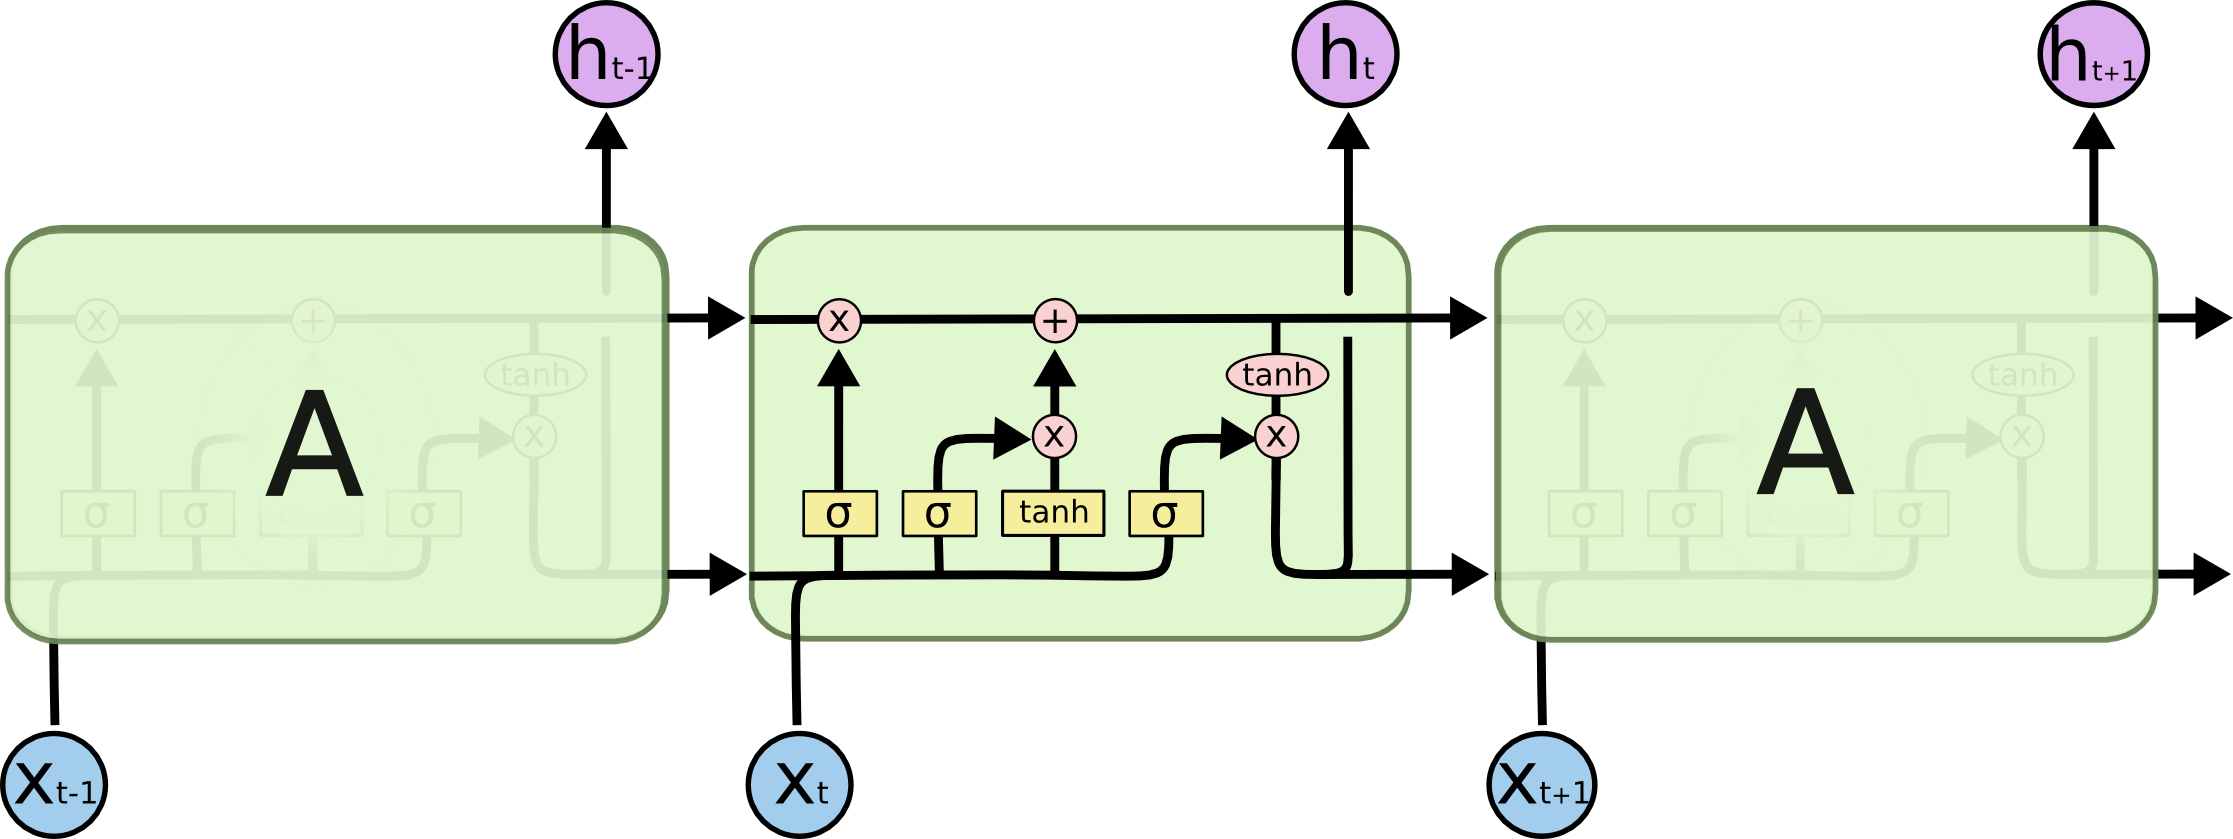
\includegraphics[scale=0.4]{LSTM.png}}
        \caption{An LSTM cell.}
        \label{fig:lstm}
    \end{figure}
    An Long Short Term Memory network (LSTM) attempts to alleviate this issue by having a "forget gate," which allows the network to select parts of an input vector to "remember" (i.e. pass on to the next cell) or "forget." It additionally has a mechanism to store and update the cell state. Let's walk through the cell step-by-step.
    \subsection{LSTM walk-through}
    \begin{figure}[H]
        \centerline{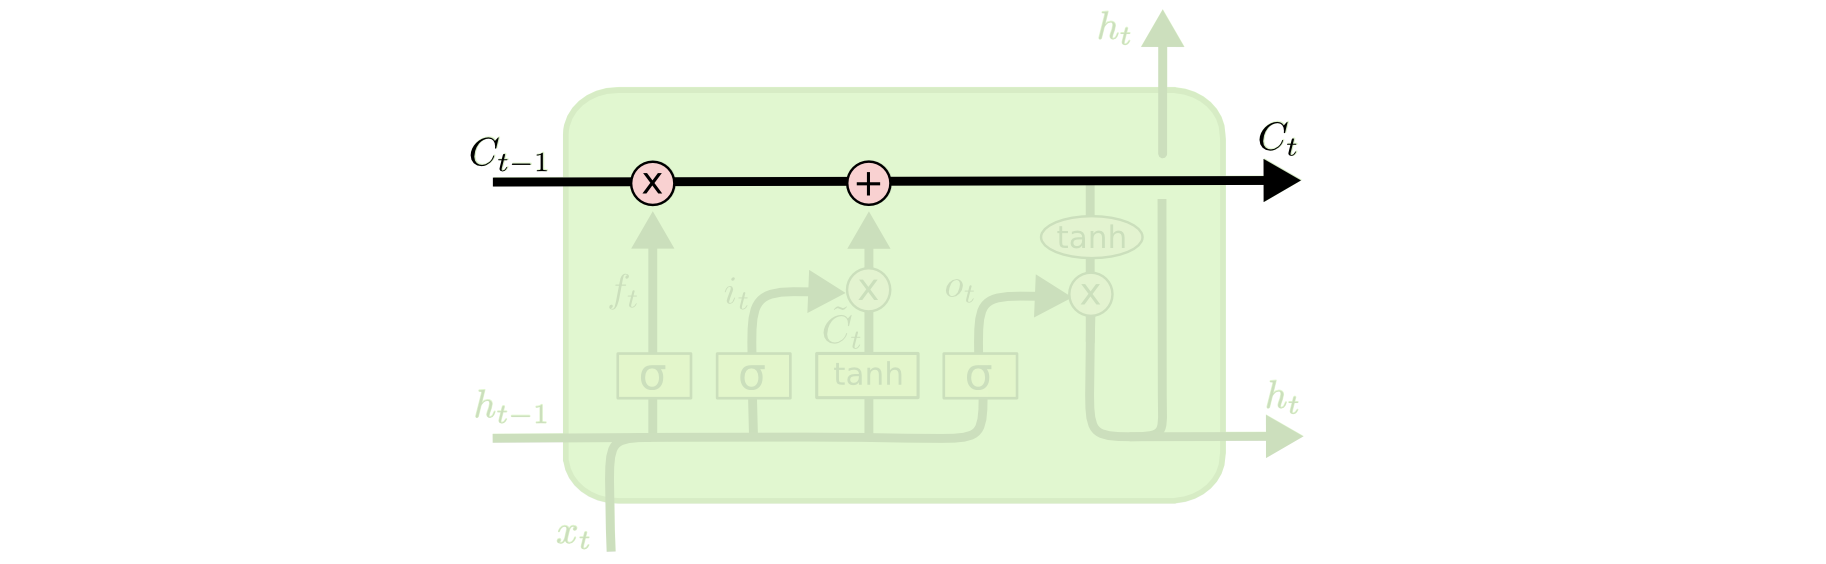
\includegraphics[scale=0.4]{LSTM0.png}}
        \caption{Cell state.}
        \label{fig:lstm0}
    \end{figure}
    First off, the cell state. This is the pathway in which information flows from cell-to-cell. It was designed so that this would have little interaction, so as to store long-term data with little change. 
    
    \begin{figure}[H]
        \centerline{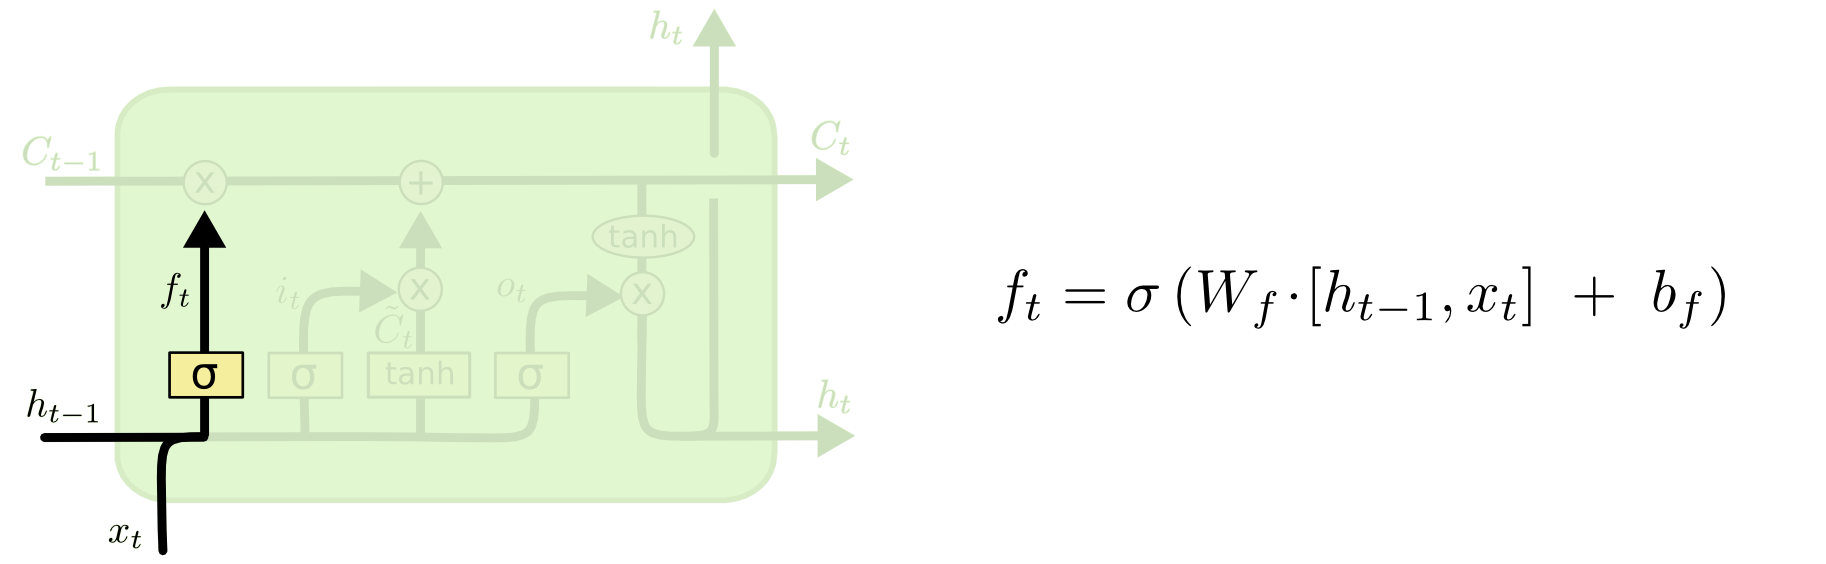
\includegraphics[scale=0.4]{LSTM1.png}}
        \caption{The forget gate.}
        \label{fig:lstm1}
    \end{figure}
    This is the forget gate. We use a sigmoid activation conditioned on the input and prior output, which gives us outputs between $0$ and $1$. Since we're multiplying this value to the cell state, an output of $0$ would correspond to completely forgetting everything, $1$ remembering everything. This is done so as to update old information with more the more recent context.
    
    \begin{figure}[H]
        \centerline{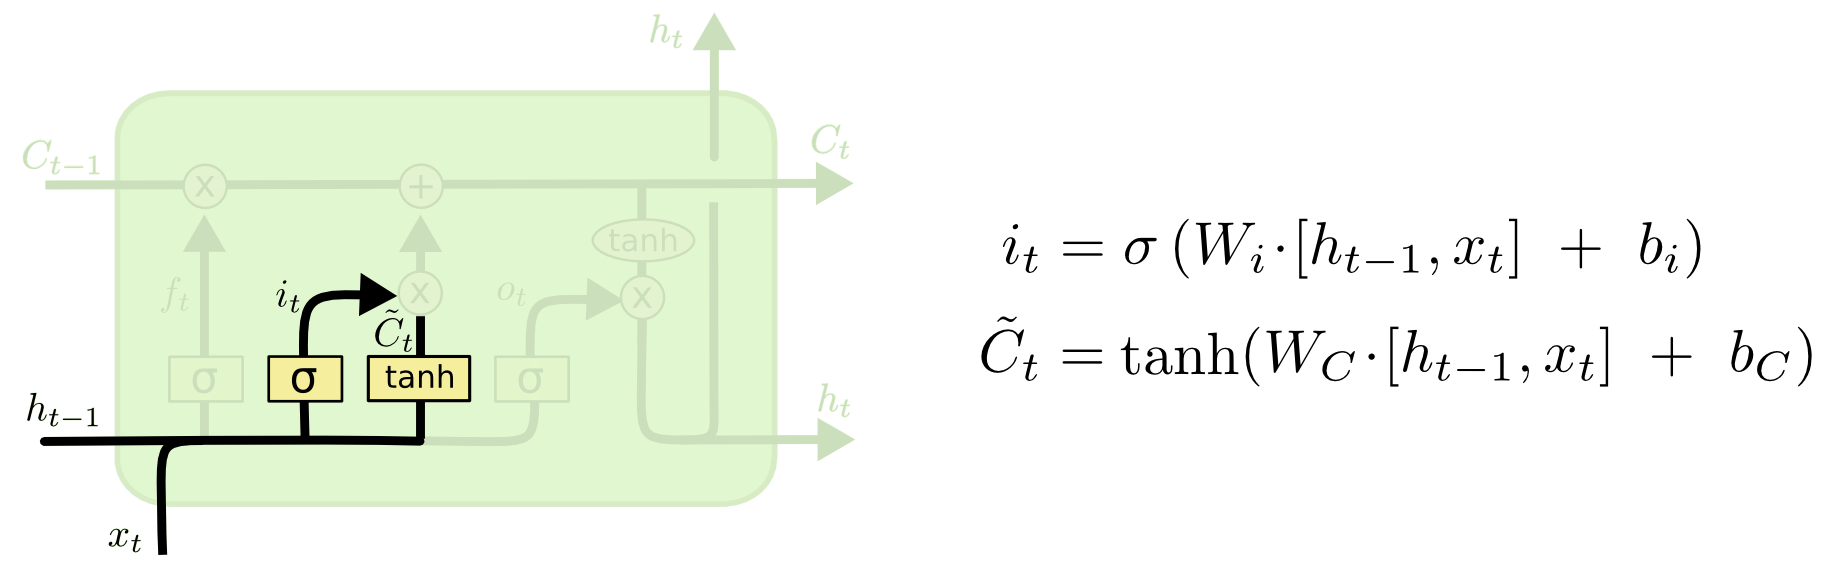
\includegraphics[scale=0.4]{LSTM2.png}}
        \caption{Updating the cell state.}
        \label{fig:lstm2}
    \end{figure}
    \begin{figure}[H]
        \centerline{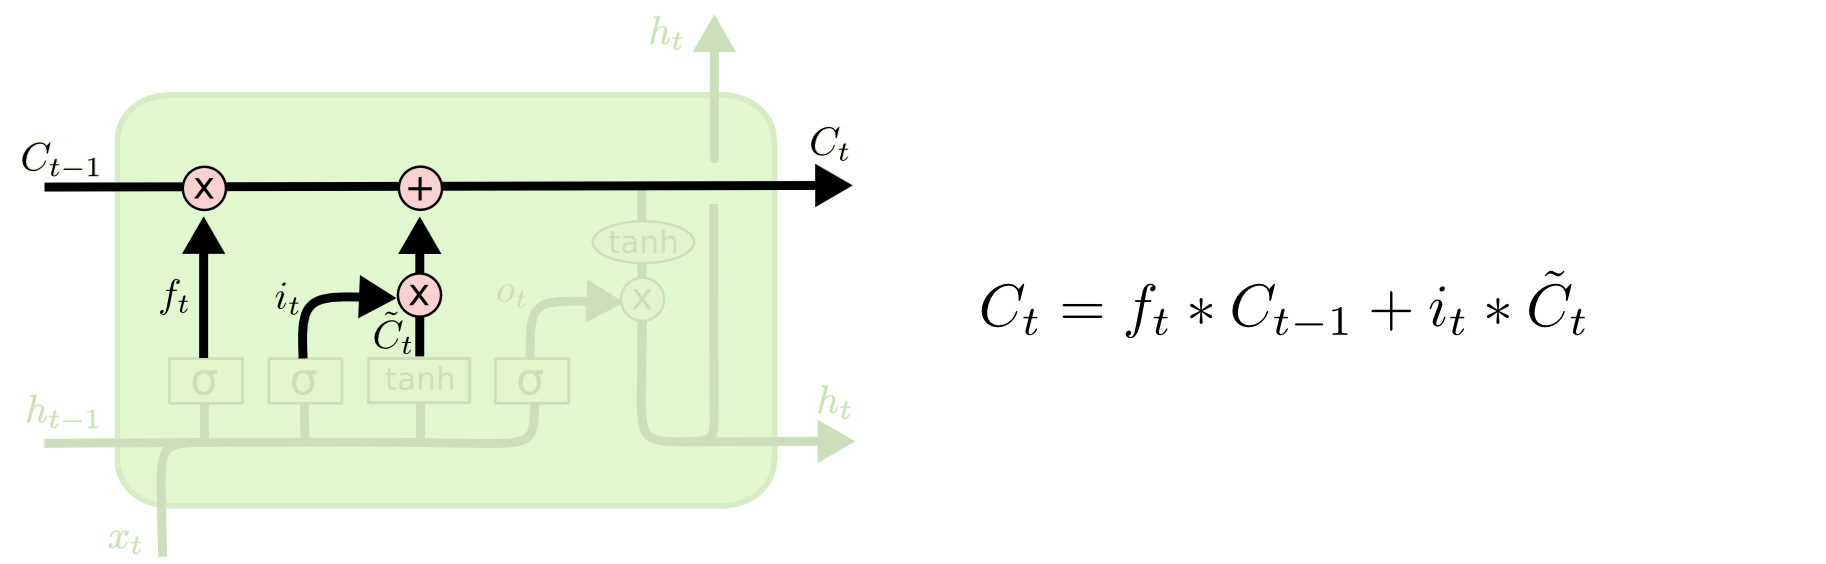
\includegraphics[scale=0.4]{LSTM3.png}}
        \caption{Outputting the cell state.}
        \label{fig:lstm3}
    \end{figure}
    Next, we add a vector to the cell state based on the input and previous output, so as to update the state. Note that we're adding values between $-1$ and $1$; $\tanh$ outputs $-1$ to $1$, and the sigmoid outputs $0$ to $1$, which determines the magnitude of the update. 
    \begin{figure}[H]
        \centerline{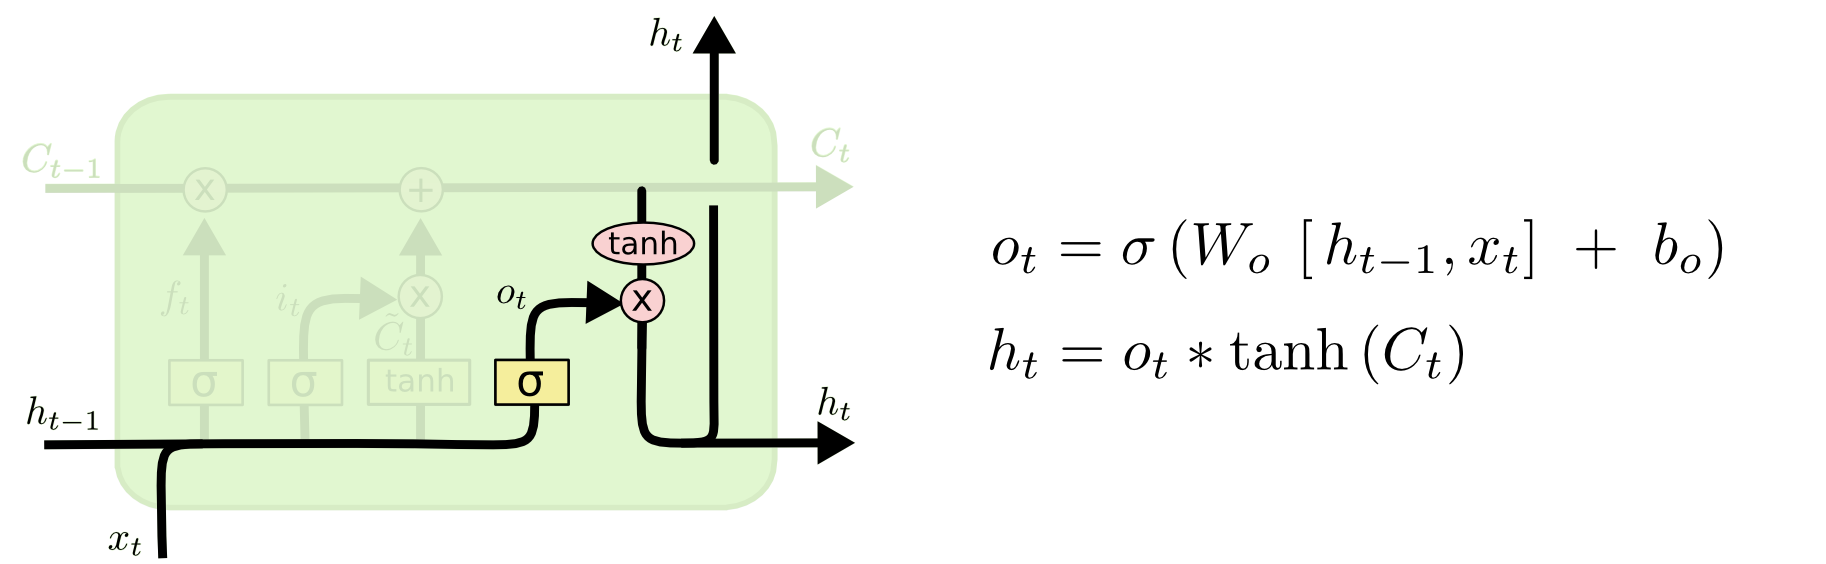
\includegraphics[scale=0.4]{LSTM4.png}}
        \caption{Outputting the final value.}
        \label{fig:lstm4}
    \end{figure}
    Lastly, we want to output $h_i$. This is determined by the cell state, which is run through $\tanh$ to bound the values between $-1$ and $1$. The sigmoid, whose output is conditioned on the previous cell output and current input, allows the cell to select which parts of the cell state to output (the sigmoid will output $0$ for the parts it does not want to output, and vice-versa). 
    
    Then, the process repeats, with the next input.
    \subsection{GRUs}
        
        \begin{figure}[H]
            \centerline{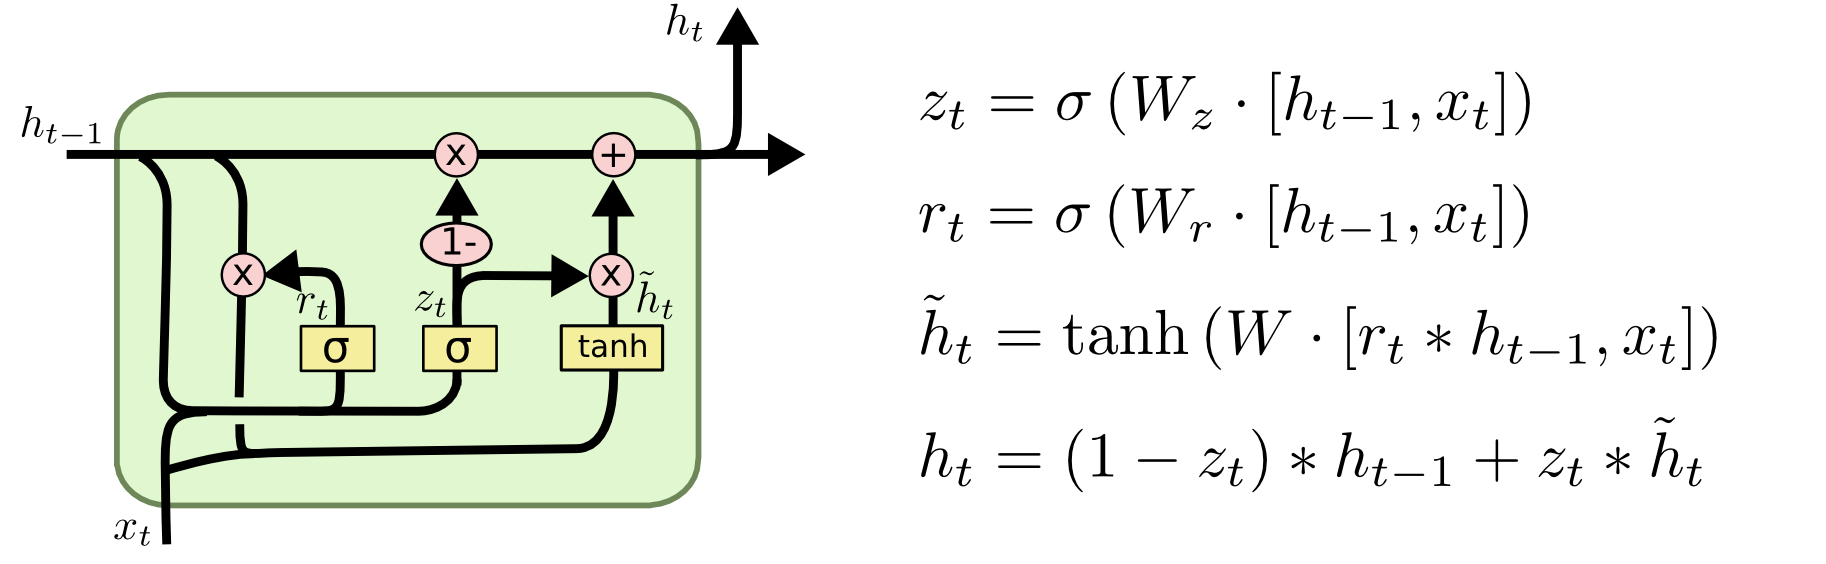
\includegraphics[scale=0.4]{GRU.png}}
            \caption{A GRU cell.}
            \label{fig:gru}
        \end{figure}
        A Gated Recurrent Unit (GRU) is an alternative to an LSTM that is computationally simpler. It opts to combine the update and forget mechanisms into an "update" mechanism, and also combines the hidden state and the cell state. GRUs are becoming increasingly popular as the perform as well as LSTMs on some tasks at a significantly lower computational cost.

\section{Conclusion}
    There are many other types of RNNs; LSTMs and GRUs are two of the most popular. Additionally, there have been advancements on RNNs themselves; "attention" mechanisms are popular in tasks such as machine translation and caption generation. 
    
    For NLP tasks, we recommend investigating word vectors (Word2Vec, skip-thought vectors, etc.) to encode words to vectors. Also, using RNNs as the basis for an encoder/decoder model is widely used to translate sequences (e.g. machine translation). We encourage you to further investigate these areas!
    
    Diagrams were obtained from [http://colah.github.io/posts/2015-08-Understanding-LSTMs/]
\end{document}
